\documentclass[preprint,3p,twocolumn]{elsarticle}
\usepackage[utf8]{inputenc}
\usepackage{amsmath}
\usepackage{amsthm} %For \newtheorem
\usepackage{amsfonts}
\usepackage{amssymb}
\usepackage{makeidx}
\usepackage{graphicx}
\usepackage{natbib}

%For algorithms
\newtheorem{algorithm}{Algorithm}[section]

\begin{document}
\begin{frontmatter}
  \title{A rules-based learning approach for generating trading strategies for the stock market}
  
  \author[1]{David Ricardo Montalván Hernández \corref{cor1}}
  \ead{davidricardo888@gmail.com}
  
  \author[1]{Salvador Godoy Calderón}
  \ead{sgodoyc@gmail.com}
  
  \address[1]{Centro de Investigación en Computación, Instituto Politécnico Nacional,
  Av. Juan de Dios Bátiz e/ M.O. de Mendizábal s/n, Nva Ind. Vallejo, 07738, Mexico City, Mexico}
  
  \cortext[cor1]{Corresponding author}
  
  \begin{abstract}
  Abstract
  \end{abstract}
  
  \begin{keyword}
  Keywords
  \end{keyword}
  
\end{frontmatter}

\section{Introduction}
\label{sec:introduction}
Introduction

\section{State of the art}
\label{sec:state of the art}
State of the art

\section{Background}
%Efficient market hyphotesis and buy & hold
%Technical indicators
%Laplace accuracy
\label{sec:background}

\subsection{AQ and CN2 algorithms}
\label{subsec:algorithms}

\subsubsection{AQ algorithm}
\label{subsubsec: aq algorithm}
The algorithm quasi-optimal (AQ), (for a thorough review of the algorithm please see \cite{michalski1969quasi}, \cite{AQMichalski1991}, \cite{AQCervone2010}, \cite{AQWojtusiak2012}), is a rule induction supervised algorithm based on the principle of separate and conquer.

Given two sets of observations $P_1, P_2, \ldots, P_n$ and $N_1, N_2, \ldots, N_m$, the positive and negatives examples respectively, AQ finds rules that are complete (cover all positive examples) and consistent (don't cover any of the negative examples).

Typically, rules are defined in the form 
$$ Consequent \leftarrow Premise \sqsubset Exception $$ 

where $Premise$ and $Exception$ are conjunctions of conditions (also called complexes) and each condition is in the form

$$ \left[Attribute.OP.Values\right]$$

where $OP$ depends on the attribute type, for example, if we are using continuous attributes, $OP \in \{ >, \geq, <, \leq  \}$.

The $Consequent$ part is typically a single condition, e.g., buy action.

The algorithm starts by selecting a positive example $e$, the seed, which is then generalized by creating all complexes that cover $e$ and do not cover any of the negative examples $N$. This set of complexes, $G(e,N)$, is called a star. The best complex in $G(e,N)$ is selected according to a user-defined criterion and added to the cover of the positive class. This process is repeated until we have a disjunction of complexes covering every positive example and none of the negative examples.

Algorithm \ref{algo:AQ} shows the pseudo-code of AQ algorithm
\begin{algorithm}[AQ algorithm]
\begin{tabbing}
\\Let $P$ be the set of positive examples of class C
\\Let $N$ be the set of negative examples of class C\\
1. \=$Cover$ $\leftarrow \emptyset $ \\
2. Repeat while $P \neq \emptyset$:\\
 \>3. Select a seed $e$ from $P$\\
 \>4. Generate a star $G(e,N)$\\
 \>5. Select the best complex, $c$, from $G(e,N)$\\
 \>6. Include $c$ in $Cover$\\
 \>7. Remove from $P$ all the examples covered by $c$\\
\=8. Return $Cover$
\end{tabbing}
\label{algo:AQ}
\end{algorithm}

\subsubsection{CN2 algorithm}
The CN2 algorithm removes AQ's dependence on specific negative examples during the star formation procedure, this is done extending the search space by examining all the possible specializations for a given complex and not just those specializations consistent with the seed and the negative examples \cite{CN2-Clark1989}.

In order to select the best complex, CN2 uses two functions for guiding the creation of the star. The first of these functions measures the quality of each complex by using information-theoretic entropy (the lower the entropy the better the complex)

\begin{equation} \label{eqn:cn2-entropy}
Entropy = - \sum_{i=1}^{n} p_{i} log_{2}(p_{i})
\end{equation}


where $n$ is the number of classes and $p_{i}$ is the probability distribution of class $i$ among all examples covered by the cover. For example for a two class problem, a complex with $P = (p_{1}, p_{2}) = (0.8, 0.3)$ means that, among all of its examples covered, $80\%$ belongs to class $1$ and $20\%$ to class 2.
Thus, using entropy, we prefer complexes that cover a large number of examples pertaining to the same class.

The second function assesses the significance of the complex by ensuring that the decisions are different from those that would result if the complex selected examples randomly. This significance is tested using the following likelihood ratio:

\begin{equation} \label{eq:cn2-ratio}
2 \sum_{i=1}^{n} f_{i} log \left( \frac{f_{i}}{e_{i}} \right) 
\end{equation}

where $f_{i}$ is the observed frequency for class $i$ among the examples covered by the complex and $e_{i}$ is the expected frequency for class $i$ under the assumption that the complex selects examples randomly.

It can be shown that the function in (\ref{eq:cn2-ratio}) is distributed approximately as $\chi^2$ with $n-1$ degrees of freedom and thus can be used as measure of statistical significance.

Algorithm \ref{algo:CN2} shows the pseudo-code of CN2 algorithm
\begin{algorithm}[CN2 algorithm]
\begin{tabbing}
\\Let $E$ be the set of examples
\\Let $S$ be the set of all selectors\\
1. \=$RULES$ $\leftarrow \emptyset $ \\
2. Repeat while $E \neq \emptyset$ or $BC \neq \emptyset$:\\
 \>3. Select the best complex $BC$\\
 \>4. Let $EC$ the examples covered by $BC$ \\
 \>5. Remove $EC$ from $E$\\
 \>6. Let $C$ the most common class in $EC$\\
 \>7. Add rule "IF $BC$ then $C$" to $RULES$\\
\=8. Return $RULES$
\end{tabbing}
\label{algo:CN2}
\end{algorithm}


\section{Proposed methodology}
\label{sec:proposed methodology}
\subsection{Data}
\label{subsec:data}
We used daily prices from the exchange-traded fund \textit{SPDR S\&P 500\footnote{Data from Yahoo Finance}} (which tracks stock index S\&P 500) for a time period comprising from 2008/01/02 up to 2019/03/06.

\subsubsection{Data split}
\label{subsubsec:data split}
In order to obtain the training and test sets, we split the data using a sliding window of 90 trading days. Our splitting criterion is motivated by the fact that using such window we are able to capture the quarterly reports of financial statements from each company in the \textit{S\&P 500}, hence we can capture how investors react to such information.

Thus, each training set comprises a 90 trading-days period which is followed by the next 90 trading-days period representing the test set. This latter set will become a the new training set and the following 90 trading-days will become a new test set and so on.

An example of our data split is represented in table \ref{table:data split}.

\begin{table}[h]
\centering
\begin{tabular}{ll}
\hline
\textbf{Training set period} & \textbf{Test set period} \\
\hline
2008/01/02 - 2008/05/09 & 2008/05/12 - 2008/09/17 \\
2008/05/12 - 2008/09/17 & 2008/09/18 - 2009/01/27 \\
2008/09/18 - 2009/01/27 & 2009/01/28 - 2009/06/05 \\
\hline
\end{tabular}
\caption{\label{table:data split} Data split}
\end{table}

Using this split methodology, we obtained $30$ training datasets ranging from $2008/01/02$ up to $2018/09/20$ and $30$ test datasets ranging from $2008/05/12$ up to $2019/01/31$.

\subsection{Attributes}
\label{subsec:attributes}
As attributes we choose a set of financial technical indicators. The motivation for its use is that such indicators are derived from experts' knowledge and thus can help us capture previously studied patterns in the data.

The technical indicators used in this work are listed next

\begin{itemize}
\item Difference of Aroon up and Aroon down, 25 days time window each.

\item Relative strength index with a 14 days window.

\item Money flow index with a 14 days window.

\item Williams \%R with a 14 days window.

\item Commodity channel index with a 20 day window and a factor $C = 0.015$
\end{itemize}

\subsection{Labelling methodology}
\label{subsec:labelling}
Since our raw data has no labels, we used an univariate marginal distribution algorithm (UMDA) in order to obtain the buy, sell and hold signals for the training data. \cite{simon2013evolutionary}.

Each individual in the population represents a particular trading strategy for the given training period. This strategy is encoded as a vector $\mathbf{x} = \left(x_1, x_2, \ldots, x_t \right)$ whose components, $x_{i}$, represent the action for the day $i$ with $ x_{i} \in \{-1,0,1 \}$, where $-1,0$ and $1$ represent sell, hold and buy signals respectively. 

The fitness function used is \textit{excess return} over the buy-and-hold strategy.

As shown in figure \ref{figure:Labelling}, this labelling methodology captures the basic intuition of "buying in lows and selling in highs".

\begin{figure}[h]
\centering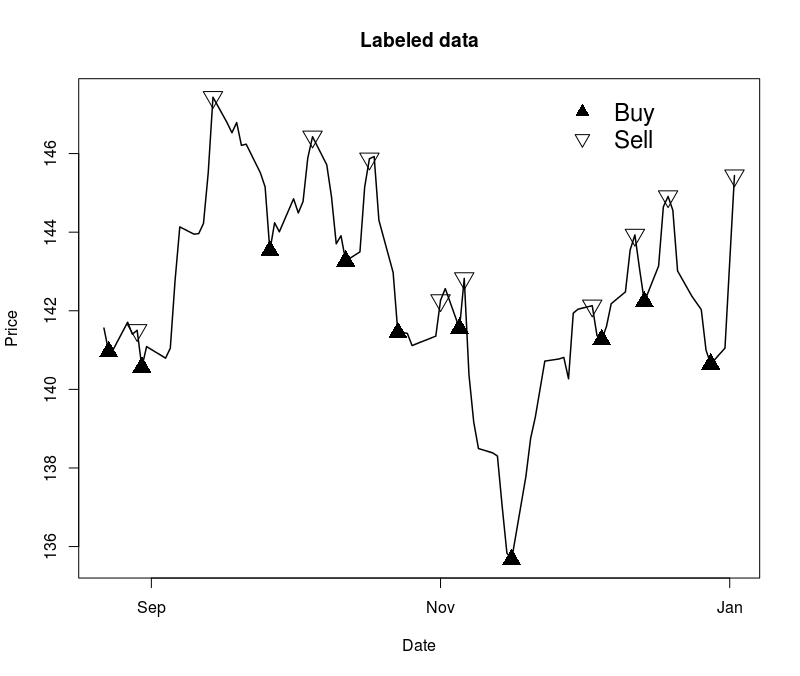
\includegraphics[width=1\linewidth]{images/labelling.jpeg}
\caption{\label{figure:Labelling} Labelled data set}
\end{figure}

\subsection{Incremental learning}
For both learning algorithms, AQ and CN2, we realized two type of experiments. The first of them is based on a \textit{learn-apply-discard} approach, in which, given a training set, we induce a set of rules and apply them to the closest test set. After that, we discard these set of rules (forget mechanism).

The other approach is based on an \textit{incremental learning} methodology, in which we learn a set of rules and instead of discarding them we order them according to their performance over the training set from which they were induced for the first time and their performance over the test sets in which they were used, keeping just a \textit{top k} of buy rules and a \textit{top k} of sell rules.

For measuring rule's performance over a training set we use the sum of their \textit{support} and their \textit{Laplace accuracy}.

On the other hand, for measuring rule's performance over a test set and in order to consider the non-stationary behaviour of stock markets, we reward (penalize) a pair of buy-sell rules, if their interaction involved a gain (loss).

The reward (penalization) given to each pair of buy-sell rules in a buy-sell transaction, is the percentage gain (loss) they caused, that is:

\begin{equation} \label{eqn:reward}
reward(B,S) = \dfrac{P_{sell} }{P_{buy}} -1 
\end{equation}

where $reward(B,S)$ is the reward (or loss) for a pair of buy-sell rules in a buy-sell transaction and $P_{sell}$, $P_{buy}$, are the sell and buy price respectively.

Finally for each rule that did not appear in the test set being evaluated, we penalize it with the average loss over that same test set, this acts as a way for discarding rules due to the pass of time.

Thus, the score for a rule, $R$, before the test set $M$, is given by:

\begin{equation} \label{eqn:rule-score}
score_{t}(R) = support + Laplace + \sum_{i} rewards_{i}
\end{equation}

where $support$ and $Laplace$ are, respectively, rule's support and its Laplace accuracy, both as measured in the training set from which it was induced for the first time. The sum in equation (\ref{eqn:rule-score}) includes all the test sets that appear after the first training set where the rule $R$ is induced and up to (excluding) the $M$-th test.

In this way, we are able to keep past and present knowledge and also identify sets of useful rules while discarding the ones that caused losses.

Figure \ref{figure:Incremental-learning} shows the process of incremental learning. For all the experiments the value of $K$ is set equal to $5$.
\begin{figure}[h]
\centering
\scalebox{0.5}{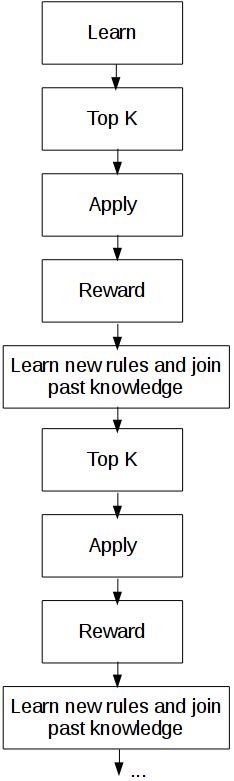
\includegraphics[width=1\linewidth]{images/incremental-learning.png}}
\caption{\label{figure:Incremental-learning} Incremental learning}
\end{figure}

\subsection{Stop loss and stop gain}
\label{subsec:stop loss and stop gain}

\subsection{Trading assumptions}
\label{subsec:trading-assumptions}
For every experiment the following trading assumptions are made:

\begin{itemize}
\item Given a buy or sell signal at time $t$, its execution is realized at time $t+1$ and the execution price is the mid price (average of low and high price) at $t+1$.

\item The transaction cost per operation is set equal to $0.25\%$. Thus for a buy transaction we end up paying:
$$ P_{buy} (1 + 0.0025)$$
per share. Whereas for a sell transaction we receive:
$$ P_{sell} (1 - 0.0025)$$ 
per share.

\item For a buy signal, we buy as many stocks as we can afford with our current capital. Likewise for a sell signal we sell all the stocks held at that time.

\item We can only sell something that we own, that is, we don't allow short sales.
\end{itemize}




\section{Results}
\label{sec:results}
Results

\section{Discussion and conclusions}
\label{sec:conclusions}
Discussion and conclusions
%Are rules financial coherent?
%Future work (other formulae for rewards)

\bibliography{references}
\bibliographystyle{elsarticle/elsarticle-harv.bst}


\end{document}